\documentclass[journal]{IEEEtran}
\usepackage{graphicx}
\usepackage[utf8]{inputenc}
\ifCLASSINFOpdf
\else
\fi
\hyphenation{op-tical net-works semi-conduc-tor}
\begin{document}
\title{Generador de Kakuros}
\author{Eduard~Torres~Chaves,~\IEEEmembership{}
        y~Juan~José~Solano~Quesada,~\IEEEmembership{}
\thanks{E. Torres Chaves estudiante de Ingeniería en computación, Instituto Tecnológico de Costa Rica}% <-this % stops a space
\thanks{J.J. Solano estudiante de Ingeniería en computación, Instituto Tecnológico de Costa Rica}% <-this % stops a space
\thanks{}}
\maketitle
\begin{abstract}
This document discusses the study of the order of functions of pruning, backtracking and the functions in charge of permuting a list. It begins with the study of the large backtracking O and backtracking itself, then follows the study of the or the functions in charge of pruning and then the function in charge of performing permutations.

\end{abstract}
\begin{IEEEkeywords}
Backtracking, thread, poda.
\end{IEEEkeywords}
\IEEEpeerreviewmaketitle

\section{Introducción}
Un kakuro es un juego matemático que consiste en un conjunto de casillas blancas y negras, en las cuales se deben rellenar las casillas blancas en el tablero con números del 1 al 9 tal que las suma de los valores en las casilla sea igual a la clave que se encuentra a la izquierda para las filas y por encima de las columnas.\\
Entre sus reglas se distinguen que no se puede repetir el valor de una casilla en la misma fila y columna hasta que haya un espacio negro y, por ende, la cantidad máxima de celdas consecutivas es 9.\\
Los problemas matemáticos que representan estos enigmas pueden resolverse utilizando tecnicas de matriz matemática y backtracking.

\begin{figure}[h] 
        \centering 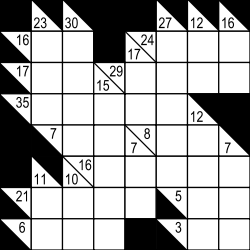
\includegraphics[width=.35\columnwidth]{kakuro_blank.png}
        \caption{
                \label{fig:samplesetup}
                Ejemplo de kakuro sin resolver
        }
\end{figure}

\begin{figure}[h] 
        \centering 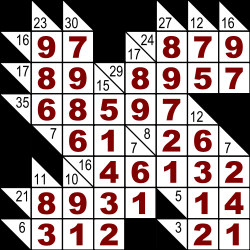
\includegraphics[width=.35\columnwidth]{kakuro_solved.png}
        \caption{
                \label{fig:samplesetup}
                Ejemplo de kakuro resuelto
        }
\end{figure}

\section{Análisis}
\subsection{Permutaciones}
En la figura 3
, se muestra la funci\'{o}n utilizada para calcular las permutaciones de una lista de tama\~{n}o $n$,  al estudiar la funci\'{o}n y las caracteristicas del mismo, se llega a la comclusion de que posee un orden de $\mathcal{O}(n!)$, ya que en la definici\'{o}n fundamental de una permutaci\'{o}n es la igual al orden del factorial de n o $!n$, este representa el número de formas distintas de ordenar $n$ objetos de manera diferente(sin repetir ordenes).El contenido de la lista se vuelve indiferente ya que, no importa el valor de los mismo a la hora de correr el algoritmo, pero si afecta el numero de los mismo.
\begin{figure}[hb] 
	\centering 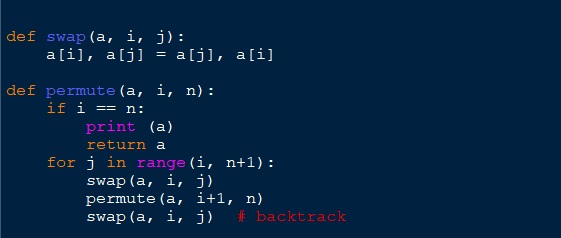
\includegraphics[width=0.9\columnwidth]{permutacion.png}
	\caption{
		\label{fig:samplesetup}
		Función de permutaciones 
	}
\end{figure} 
\subsection{Poda}
\subsection{Backtracking}
Al momento de analizar las funcio\'{o}nes encargadas del backtraking, se debe de tomar en cuenta que el orden puede ser afectado por otras funci\'{o}nes, como por ejemplo las encargadas de la poda, sin embargo, al ser estudiadas en otra secci\'{o}n, no se contemplara el efecto que tengan en el orden del backtracking.\\
El kakuro tiene la particularidad de solo tener, por numero, 9 casillas vaci\'{a}s, por lo que el rango maximo de interaciones por numero a calcular es de 9.\ La funci\'{o}n backtrack, figura 4, busca la solucion con un maximo de 11 veces por el parametro "intentos" (maximo de veces que un mismo numero aparece en una lista de los posibles conjuntos) si no es que no ha encontrado una soluci\'{o}n, al analizarla obtenemos un orden $O(n^(11))$ pero a su vez, backtrack llama a la funci\'{o}n meterEnMatriz, figura 5, por lo que es necesario el estudio de la funci\'{o}n meterEnMatriz.
\\
La funci\'{o}n meterEnMatriz entra en un while que puede tener dos duraciones, en el mejor caso una duraci\'{o}n de 9 (en el caso de ser una serie de 9 espacios en blanco sin ninguna intersecci\'{o}n) o de 15 como maximo de interaciones antes de que se requiera otro grupo de soluci\'{o}n (el cual se encarga la funci\'{o}n backtrack), por lo que el orden de la funci\'{o}n esta dada por $O(15)$ al ser 15 el maximo entre (9,15).\\ 
\begin{figure}[h] 
	\centering 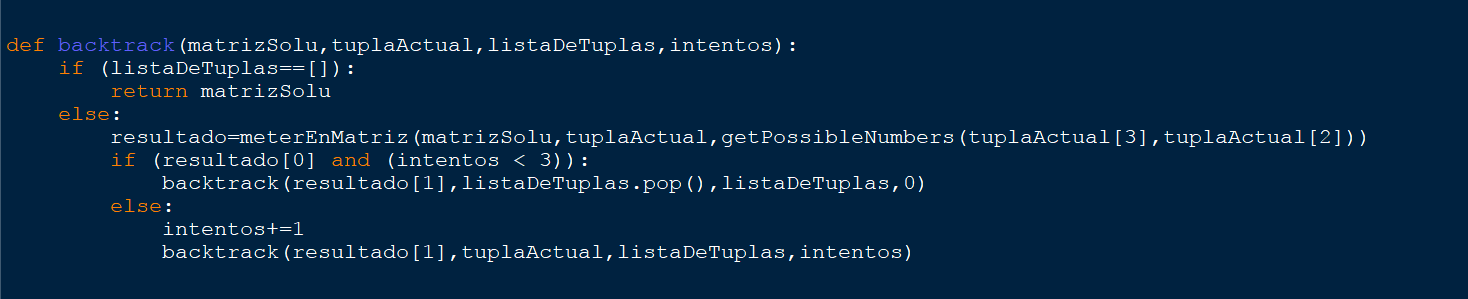
\includegraphics[width=1\columnwidth]{backtrack_parte1.png}
	\caption{
		\label{fig:samplesetup}
		Función de Backtrack
	}
\end{figure}
\begin{figure}[h] 
	\centering 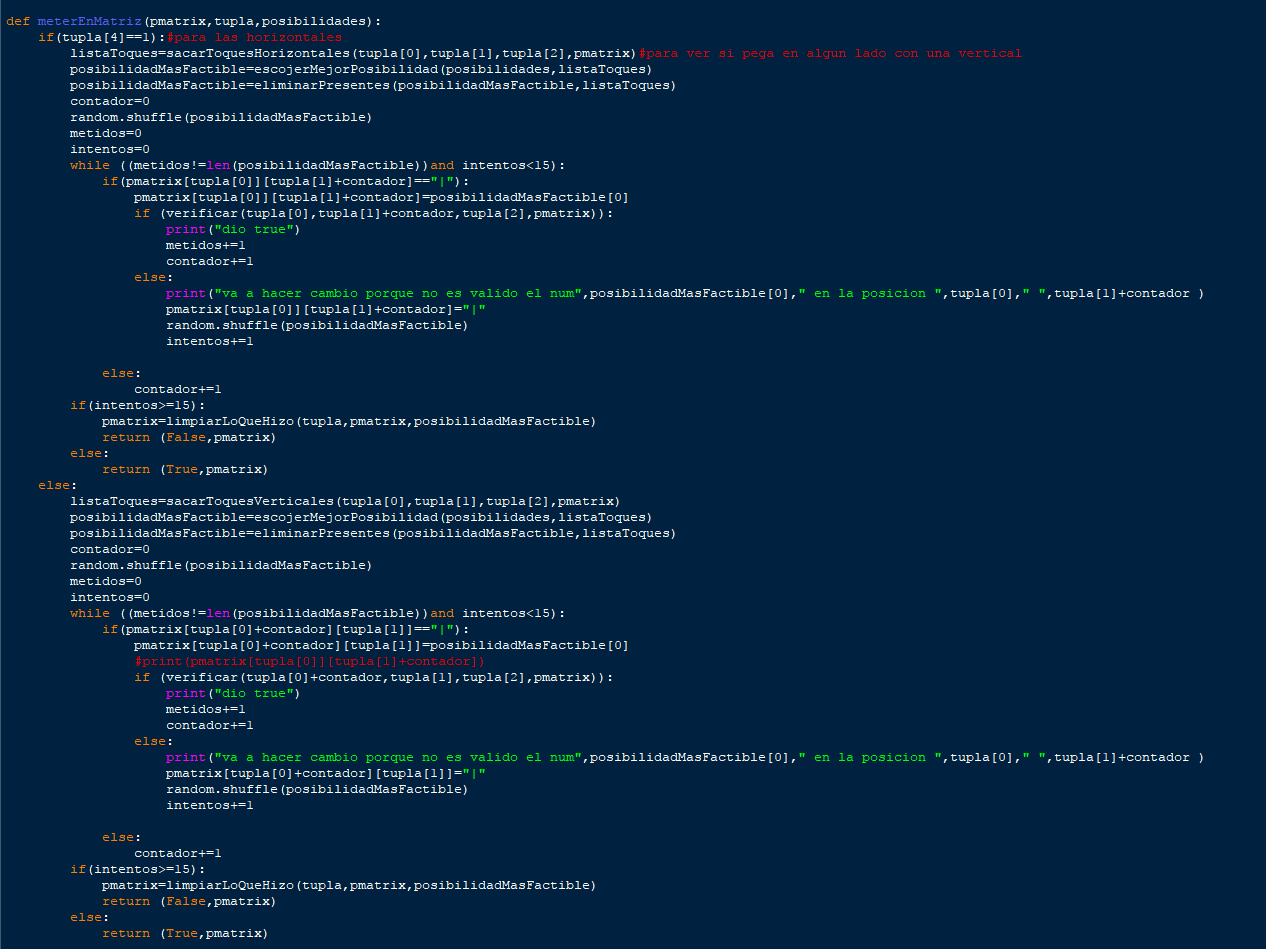
\includegraphics[width=1\columnwidth]{backtrack_parte2.png}
	\caption{
		\label{fig:samplesetup}
		Función de meterEnMatriz
	}
\end{figure}
\subsection{Generar un tablero}


\end{document}